\documentclass[11pt,aspectratio=169]{beamer}
\usepackage[T1]{fontenc}
\usepackage[utf8]{inputenc}
\usepackage{lmodern}
\usepackage{booktabs,tabularx}
\usepackage{graphicx}
\usepackage{amsmath, amssymb, amsfonts, amsthm, bbm}
\usepackage[
    natbib=true,
    bibencoding=inputenc,
    bibstyle=authoryear-ibid,
    citestyle=authoryear-comp,
    maxcitenames=3,
    maxbibnames=10,
    useprefix=false,
    sortcites=true,
    backend=bibtex
]{biblatex}
\AtBeginDocument{\toggletrue{blx@useprefix}}
\AtBeginBibliography{\togglefalse{blx@useprefix}}
\setlength{\bibitemsep}{1.5ex}
\addbibresource{References.bib}

\usepackage{hyperref}
\hypersetup{
    colorlinks=true,
    linkcolor=black,
    anchorcolor=black,
    citecolor=black,
    filecolor=black,
    menucolor=black,
    runcolor=black,
    urlcolor=black}

\DeclareMathOperator{\argmax}{arg\,max}

%Theorem
\newtheorem{assumption}{Assumption}
\newtheorem{proposition}{Proposition}
\newtheorem{defn}{Definition}
\newtheorem{LEMmA}{Lemma}


\begin{document}
\mode<presentation>{	
    \setbeamertemplate{navigation symbols}{}
}

\title{Topics in Behavioral Decisons in Finance}
\date{Discussion by Christian Hilpert\\ \today}
\begin{frame}
    \titlepage
\end{frame}

\begin{frame}{5. Alternative Theories of Choice under Risk}
    {5.1 Reference-Dependent Risk Attitudes}
\textbf{Kőszegi, Rabin (2007, AER)}
    \begin{itemize}
 
        \item choice of reference point in CPT exogenous.\medskip
        \item has huge impact for economic choices\medskip
        \item $\Rightarrow$ literature on disposition effect\medskip
        \item new model:\medskip
        \begin{itemize}
            \item combines gain/loss utility with standard consumption utility \medskip
            \item Rabin(2000):(50/50, +550,-500) $\Rightarrow (+100,000,000,000,000, -4,000) \Rightarrow $ reject\medskip
            \item endogenously determines reference point\medskip
            \item allows for stochastic reference points.\medskip
        \end{itemize}

	\end{itemize}
\end{frame}

\begin{frame}{5.1 Reference-Dependent Risk Attitudes}
    \begin{enumerate}
        \item surprise, low probability decisions, exogenous expectations; say pay \$55 to insure \$100 risk, 50\%\medskip
        \begin{enumerate}[(a)]
            \item status quo:0. $\rightarrow$ diminishing sensitivity do not insure\medskip
            \item expect to pay 55: lose 45 gain 55 . loss aversion $\rightarrow$ insure.\medskip
        \end{enumerate}
        \item anticipated risks
        \begin{enumerate}[(a)]
            \item macdimahing personal equilibrium (UPE)\\
            behaviour where the stochastic outcome generated by utility-maximizing choices conditional on expectations equals expectations. i.e. follows planned behavior\\
            $\Rightarrow$ selects preferred personnal equilibrium (PPE)\medskip

            \item choice-acclimating personal equilibrium(CPE)\\
            committed decision long before outcomes $\Rightarrow$ reference point influenced by choice.\\
            maximize expected utility given that if determines reference lottery and outcome lottery.\medskip
        \end{enumerate}
        \item 1\&2 : linear consumption utility\medskip
        $\Rightarrow$ small gambles.\\
        now large gambles, consumption utility non-linear  $\Rightarrow$ reference point not very important.
    \end{enumerate}
\end{frame}


\begin{frame}{Model}
    \begin{itemize}
        \item $ w \in \mathbb{R}$ wealth,$r \in \mathbb{R} $ reference:\\
        $ U(w | r)=m(w)+\mu(m(w)-m(r))^2$\medskip
        \item reference point: belief of outcomes, $g $ probility measure\\
         $U(w | g)=\int u(w|r)  \,dg(r)$\\$  \Rightarrow$ mixed feelings, $50:50  0/100; 50$:gain to 0, loss to 100.\medskip
        \item $w $ has measure $F$\\
        $U(F|g)=\iint u(w|r) dg(r) dF(w) $, no probability weighting for simplicily.\medskip

	\end{itemize}
\end{frame}

\begin{frame}{Assumptions on $\mu$}  
    \begin{itemize}
        \item A0: $\mu(x) $ continuous , twice differentiable for $x\neq 0, \mu(0)=0 $.\medskip
        \item A1: $ \mu(x)$ strictly increasing. \medskip
        \item A2: if $y>x\geq 0 $, then $\mu(y)+\mu(-y) <\mu(x) +\mu(-x) $.\medskip
        \item A3: $ \mu^{"}(x) \leq 0 $ for $ x>0$ and $\mu^{"}(x) \geq 0$ for $ x<0 $.\medskip
        \item A4: $\frac{\mu^{'}_{-}(0)}{\mu^{'}_{+}(0)} \equiv \lambda >1 $, \\
    where $ \mu^{'}_{+}(0) \equiv \lim_{x \to 0} \mu^{'}(\left\lvert x \right\rvert )$ and $ \mu^{'}_{-}(0) \equiv \lim_{x \to 0} \mu^{'}(-\left\lvert x \right\rvert )$.\medskip
        \item A2,A4: loss aversion \medskip
        \item A3: diminishing sensitivity\medskip
        \item A3': $\forall x \neq 0, \mu^{"}(x)=0 \Rightarrow $ no diminishing sensitivity.\medskip
        \item general assumption, reference point $\neq $ expectations;rational expectations, generally people have some idea how they behave and their own environment.\medskip
	\end{itemize}
\end{frame}

\begin{frame}{1. Risk aversion in surprise situations}
    \begin{itemize}
        \item $m$ is linear: $m(w)=w$\medskip
        \item reference point fixed\medskip
	\end{itemize}
    \begin{proposition}[1]
        Suppose $m(\cdot)$ is linear and $\mu(\cdot)$ satisfies A3'(no diminishing sensitivity). For any lotteries $F,G,H$, and constant $w$,
        if $ U(w+F|g) \geq U(w|w)$, the $U(H+F|G) \geq U(H|G)$.\\
    \end{proposition}
    $\Rightarrow$
    \begin{itemize}
        \item If willing to accept F relative to riskless r, positive values of F are gains, negative ones are lossed.\medskip
        \item If F is added to lottery H relative to lottery G, positive outcomes of F eliminate losses from H relative to G, losses from F merely eliminate gains from H.\medskip
        \item $\Rightarrow$ more willing to accept F.\medskip
        \item If $H=w, G=F \quad \Rightarrow$  less risk averse in eliminating risk that is expected.\medskip
	\end{itemize}
\end{frame}

\begin{frame}{1. Risk aversion in surprise situations}
    \begin{proposition}[2]
        Suppose $m(\cdot)$ is linear. For any lottery F with positive expected value:
        \begin{enumerate}[(i)]
            \item There exist $A, \varepsilon >0 $ such that if G has $\Pr_G[r \in (k-A, k+A)]< \varepsilon $ for all constants k, then $U(H+F|G)> U(H|G)>U(H-F|G)$ for any lottery H.\medskip
            \item For any continuously distributed lottery G, there is a $\bar{t}>0 $ s.t. for any $t \in (0,\bar{t}]$ and any lottery $H, U(H+t\cdot F|G)> U(H|G)> U(H-t \cdot F|G)$.\medskip
        \end{enumerate}
    \end{proposition}
Identifies attitudes towards F in which risk neutral.\\
    \begin{enumerate}[(i)]
        \item If sufficiently widely distributed reference lottery, accept F, and reject -F.\medskip
        \item If fixed continuously distributed reference lottery, accept sufficiently small multiple of F, reject the same multiple of -F.\medskip
    \end{enumerate}
Prop. 1\&2 do not imply no risk aversion, just lower risk aversion!
\end{frame}

\begin{frame}{2. UPE and PPE Risk Attitudes}
    \begin{itemize}
        \item now correctly anticipates choice set. \medskip
        \item connot commit to choice untill shortly before outcome\\
        $L=\{D_1,1-q;D_2,q\}, D_1,D_2 \in \bigtriangleup (\mathbb{R})$\medskip
        \item for now $q=0 \Rightarrow$ choice set is certain\medskip
        \item beliefs are set, reference point exogenous.\medskip
	\end{itemize}
    \begin{definition}[UPE]
        A selection $F_1 \in D_1, F_2 \in D_2$ is an unacclimating personal equilibrium (UPE) if for each $l \in 1,2$ 
        and any $F_l^{\prime} \in D_l$, $U\left(F_l \mid(1-q) F_1+q F_2\right) \geq U\left(F_l^{\prime} \mid(1-q) F_1+\right.$ $\left.q F_2\right)$.
    \end{definition}
    (Koszegi, 2005 proves existence.)
    \begin{itemize}
        \item  If the person expects to choose $F_1$ and $F_2$ from choice sets $D_1$ and $D_2$, then she expects the distribution of outcomes $(1-q) F_1+q F_2$.\medskip
        \item Def. 1: If this is the expectation. she should be willing to choose  $F_1$ and $F_2$.\medskip
    \end{itemize}
\end{frame}

\begin{frame}{2. UPE and PPE Risk Attitudes}
Example:\\
wealth w, $50/50$ chance $0,-100$ or pay $-55$, when is the lottery a UPE?\\
$$
\begin{aligned}
{\left[\frac{1}{2}(w\right.} & \left.-100)+\frac{1}{2} w\right] \\
& +\left[\frac{1}{4} \mu(100)+\frac{1}{4} \mu(-100)\right] \\
\geq & {[w-55] } \\
+ & {\left[\frac{1}{2} \mu(45)+\frac{1}{2} \mu(-55)\right] }
\end{aligned}
$$
    \begin{itemize}
        \item UPE generally not unique.\medskip
        \item expectation: plan what to do at the time.\medskip
        \item idea: select best plan she will follow through on.\medskip
    \end{itemize}
\end{frame}

\begin{frame}{2. UPE and PPE Risk Attitudes}
    \begin{definition}[PPE]
        A selection $F_1 \in D_1, F_2 \in D_2$ is a preferred personal equilibrium(PPE) if it is a UPE, 
        and $U\left((1-q) F_1+q F_2 \mid(1-q) \mathrm{F}_1+qF_2\right) \geq U\left((1-q) \mathrm{F}_1^{\prime}+q \mathrm{~F}_2^{\prime} \mid(1-q) \mathrm{F}_1^{\prime}+q \mathrm{~F}_2^{\prime}\right)$ 
        for all $U P E$ selections $F_l^{\prime} \in D_1, F_2^{\prime} \in D_2$.\\
    \end{definition}
$\Rightarrow$ choice optimal given expectations!\\
\end{frame}

\begin{frame}{2. UPE and PPE Risk Attitudes}
    \begin{proposition}[3] 
    Suppose $m(\cdot)$ is linear. For any $w \in \mathbb{R}$ and mean-zero lottery $F \neq 0$ with bounded support, 
    there exist $\bar{k}, \bar{t}>0$ such that for any positive $t<\bar{t}, k<\bar{k}$, 
    the unique $P P E$ with the choice set $\{w, w+t(F+k)\}$ is to choose w.\\
    \end{proposition}
    \begin{itemize}
        \item select riskless w over a sufficiently small, better-than-fair but unattractive bet.\medskip
        \item loss aversion makes gamble unattractive.\medskip
        \item key point: CPT: costs $\neq $ loss in status quo.\\
        here: expected costs, such as insurance premium is a cost, not a loss.\medskip
        \item $\Rightarrow $ explain insurance for likely events  \medskip
	\end{itemize}
    \hspace*{\fill} \\  
\end{frame}

\begin{frame}{2. UPE and PPE Risk Attitudes}
    \begin{proposition}[4] 
        Suppose $m(\cdot)$ is linear, $\mu(\cdot)$ satisfies A3'. \\
        If $w+F$ is a PPE in the choice set $\{w, w+F\}$, then for any lottery $H$, $U(w+F \mid H)>U(w \mid H)$.\\
    \end{proposition}
    $\Rightarrow$ If choose between risk and insurance, at least a risk aversion as ????\\
    $\Rightarrow$ in experiments , people generally are in surprise settings / don't know what comes\\
    $\Rightarrow$ underestimate risk aversion\\
    Additionally (see papers) expecting risk decreases risk aversion.
\end{frame}

\begin{frame}{3. CPE Risk Attitudes}
    \begin{itemize}
        \item long commited choices\medskip
	\end{itemize}
    \begin{definition}[CPE]
        For any choice set $D, F \in D$ is $a$ choice-acclimating personal equilibrium $(C P E)$ 
        if $U(F \mid F) \geq U\left(F^{\prime} \mid F^{\prime}\right)$ for all $F^{\prime} \in D$.
    \end{definition}
    $\Rightarrow$ selecting $F$ determines it as reference point.\\
    Example:\\
    lottery $50/50$ with (0,-100) is CPE if:\\
    $$
    \begin{aligned}
    & \quad\left[\frac{1}{2}(w-100)+\frac{1}{2} w\right] \\
    & \quad+\left[\frac{1}{4} \mu(100)+\frac{1}{4} \mu(-100)\right] \\
    & \geq[w-55]+[0] .
    \end{aligned}
    $$
    \begin{itemize}
        \item UPE: premium 55 can be gain or loss;\medskip
        \item CPE: premium 55 is neither gain nor loss.\medskip
	\end{itemize}
\end{frame}

\begin{frame}{3. CPE Risk Attitudes}
Some implications:
    \begin{itemize}
        \item unlike as UPE,PPE, for CPE pepple may want to choose stochastialy dominated options\medskip
        \item idea: give up unlikely gain to avoid losses\medskip
	\end{itemize}  
\end{frame}

\begin{frame}{5.2 Salience Theory}
    \textbf{Bordalo, Gennaioli, Shleifer (2012,QJE)}   
    \begin{itemize}
        \item risk preferences not stable\medskip
        \item Allais (1953) paradoxes:irrelevant choice implies risk lottery behavior.\medskip
        \item idea: salience to prominent outcomes\medskip
        \item building blocks:
        \begin{itemize}
            \item ordering\medskip
            \item diminishing sensitivity\medskip
            \item salience weighting ($\neq$ probility weighting)
        \end{itemize}
        \item say consumer choice: speed, price, design\medskip
	\end{itemize} 
\end{frame}

\begin{frame}{5.2 Salience Theory}
\textbf{Allais (1953) paradoxes}\\
$L_1(z)=\left\{\begin{array}{lll}\$ 2500 & \text { with prob. } & 0.33\\ \$0 & & 0.01 \\ \$ z & & 0.66\end{array}\right.$\\
\hspace*{\fill} \\ 
$L_2(z)=\left\{\begin{array}{lll}\$ 2400 & \text { with prob. } & 0.34 \\ \$ z & & 0.66\end{array}\right.$\\
In experiments: $z=2400$ \\
\hspace*{\fill} \\ 
$$
L_1(2400)= \begin{cases} 2500 \text { with prob. } & 0.33 \\  0 & 0.01 \prec  L_2(2400)=2400\\  2400 & 0.66\end{cases}
$$
$\Rightarrow$ risk averse
\end{frame}

\begin{frame}{5.2 Salience Theory}
In experiments: $z=0$ \\
$L_1(0)= \begin{cases} 2500 \text { with prob. } & 0.33 \\ 0 & 0.67 \end{cases}$ $\succ$
$L_2(0) = \begin{cases} 2400 \text { with prob. } & 0.34 \\ 0 & 0.66\end{cases}$\\

$\Rightarrow$ risk loving

\begin{itemize}
    \item CPT: in last gamble $w(p=0.01)$ overweighted\medskip
    \item Salience theory: $L_1(2400),L_2(2400) \rightarrow$ 2500 only slightly higher than 2400; 0 a lot lower than 2400.\medskip
    \item Salience theory: $L_1(0),L_2(0) \rightarrow$ outcome zero is standard; 2500 stands out more.\medskip 
\end{itemize}
\end{frame}

\begin{frame}{Model}
    \begin{itemize}
        \item $s \in S$: state\medskip
        \item $\pi_s$: probability, s.t. $\sum_{s \in S} \pi_s=1$\medskip
        \item $\left\{L_1, L_2\right\}$: choice set\medskip
        \item $x_s^i$: payoffs\medskip
        \item value function as before, reference dependent $V$ without decision weights, only local thinking:\medskip
        $$
    V\left(L_i\right)=\sum_{s \in S} \pi_s v\left(x_s^i\right) .
    $$
        \item With salience distortion:\medskip
        \item two steps: salience ranking, then decision weight $\pi_s^i$\medskip
        \item Formally: $\mathrm{x}_s=\left(x_s^i\right)_{i=1,2}$, payoffs in state $s$\medskip
        \item $x_s^{-i}$: payoff of lottery $L_j$, $j \neq i$\medskip
        \item $x_s^{\min }, x_s^{\max }$: largest / smallest payoffs in $\mathrm{x}_s$
	\end{itemize}
\end{frame}

\begin{frame}{Model}
    \begin{definition}[1]
        The salience of state $s$ for lottery $L_i, \mathrm{i}=1,2$, is a continuous and bounded function $\sigma\left(x_s^i, x_s^{-i}\right)$ that satisfies three conditions:\\
        \begin{itemize}
            \item 1. Ordering. If for states $s, \tilde{s} \in S$ we have that $\left[x_s^{\min }, x_s^{\max }\right] \in \left[x_{\tilde{s}}^{\min }, x_{\tilde{s}}^{\max }\right]$, then
    $$
    \sigma\left(x_s^i, x_s^{-i}\right)<\sigma\left(x_{\tilde{s}}^i, x_{\tilde{s}}^{-i}\right) .
    $$ 
            \item 2. Diminishing sensitivity. If $x_s^j>0$ for $j=1,2$, then for any $\epsilon>0$,
$$
\sigma\left(x_s^i+\epsilon, x_s^{-i}+\epsilon\right)<\sigma\left(x_s^i, x_s^{-i}\right) .
$$
            \item 3. Reflection. For any two states $s, \tilde{s} \in S$ s.t. $x_s^j, x_{\tilde{s}}^j>0, (j=1,2)$, we have\\
            $\sigma\left(x_s^i, x_s^{-i}\right)<\sigma\left(x_{\tilde{s}}^i, x_{\tilde{s}}^{-i}\right)$\\
            if and only if $\sigma\left(-x_s^i,-x_s^{-i}\right)<\sigma\left(-x_{\tilde{s}}^i,-x_{\tilde{s}}^{-i}\right)$.
        \end{itemize}
    \end{definition}
\end{frame}

\begin{frame}{Model}
    \textbf{Example:}\\
    $$
    \sigma\left(x_s^i, x_s^{-i}\right)=\frac{\left|x_s^i-x_s^{-i}\right|}{\left|x_s^i\right|+\left|x_s^{-i}\right|+\theta}, \theta>0
    $$ 
    \begin{itemize}
        \item ordering: salience rises if distance of  $x_s^i$ and $x_s^{-i}$ rises\medskip
        \item diminishing sensitivity: as average payoff gets farther from zero, salience reduces $\left|x_s^1\right|+\left|x_s^2\right|$\medskip
        \item reflection: salience is shaped by the magnitude, not sign\medskip
        \item (example: symmetric additional dropped for $N>2$)\medskip
        \item Results mostly driven by ordering and diminishing sensitivity.\medskip
	\end{itemize}
\end{frame}

\begin{frame}
    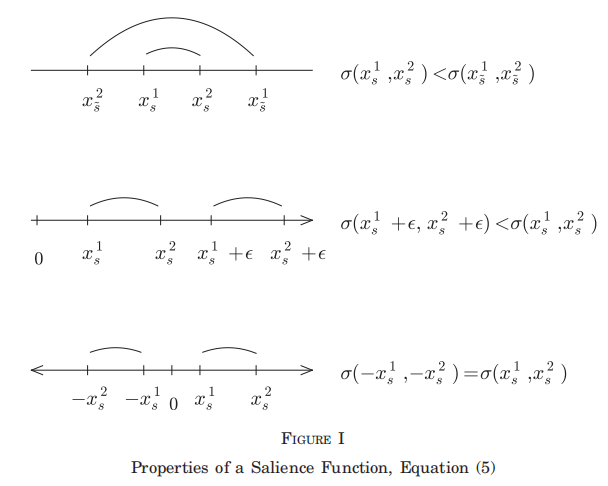
\includegraphics[width = 0.75\textwidth]{fig1.png}
\end{frame}

\begin{frame}{Model}
    \begin{definition}[2]
        Given states $s, \tilde{s} \in S$, we say that for lottery $L_i \mathrm{~s}$ $s$ is more salient than $\tilde{s}$ if $\sigma\left(x_s^i, x_s^{-i}\right)>\sigma\left(x_{\tilde{s}}^i, x_{\tilde{s}}^{-i}\right)$. 
        Let $k_s^i \in\{1, \ldots,|S|\}$ be the salience ranking of state $s$ for $L_i$, with lower $k_s^i$ indicating higher salience. 
        All states with the same salience obtain the same ranking(no jumps). Then the local thinker transforms the odds $\frac{\pi_{\tilde{s}}}{\pi_s}$ of $\tilde{s}$ relative to $s$ into the odds $\frac{\pi_s^i}{\pi_s^i}$, given by:
        $$
        \frac{\pi_{\tilde{s}}^i}{\pi_s^i}=\delta^{k_{\tilde{s}}^i-k_s^i} \cdot \frac{\pi_{\tilde{s}}}{\pi_s}, \text{\quad where } \delta \in(0,1]
        $$
        By normalizing $\sum_s \pi_s^i=1$ and defining $\omega_s^i=\frac{\delta^{k_s^i}}{\left(\sum_r \delta^{k_r^i} \cdot \pi_r\right)}$ \\
        the decision weight is: $\pi_s^i=\pi_s \cdot \omega_s^i$\\
        $\Rightarrow$ local thinker overweights most salient states. 
    \end{definition}
\end{frame}

\begin{frame}{Model}
    \begin{itemize}
        \item $\delta=1 \Rightarrow$ standard model, $\omega_s^i=1$\medskip
        \item $\delta<1 \Rightarrow$ local thinker\medskip
        \item state $s$ is overweighted, if $\left(\omega_s^i>1\right.$, or $\left.\delta^{k_s^i}>\sum_r \delta_r^{k_r^i} \cdot \pi_r\right)$\medskip
        \item $\delta \rightarrow 0$: decision based on most salient state\medskip
        \item $\delta$ is independent of objective state probabilities!\medskip
    \end{itemize}
\end{frame}

\begin{frame}{Some remarks:}
    \begin{itemize}
        \item weighting depends on salience, not low-probability\medskip
        \item low-probility can be most overweighted, but also underweighted\medskip
        \item choice of state space / atternative lottery unclear\medskip
        \item some cases: no atternative $\Rightarrow$ take zero? Open question\medskip
    \end{itemize}
\end{frame}

\begin{frame}{Risk attitudes:}
        \begin{itemize}
            \item suppose linear value function\medskip
            \item $L_0=(x,1)$: sure prospect \medskip
            \item $L_1=\left(x+g, \pi_g ; x-l, 1-\pi_g\right)$, with $g \pi_g=\left(1-\pi_g\right) l$: mean preserving spread, $x,g,x-l >0$\medskip
            \item $s_g=(x+g, x), s_l=(x-l, x)$, :two states\medskip
            \item $ V^{LT}(L)=\sum_{s \in S} \pi^i_s v\left(x_s^i\right)=\sum_{s \in S} \pi_s \omega ^i_s v\left(x_s^i\right)$\medskip
        \end{itemize}
    \end{frame}

\begin{frame}{Risk attitudes:}
    \begin{itemize}
        \item $\delta<1 \Rightarrow$ prefer $L_1$ if $s_g$ more salient, $\sigma(x+g, x)>\sigma(x-l, x)$\medskip
        \item  Using $g \pi_g=\left(1-\pi_g\right) l$, $\sigma\left(x+\frac{1-\pi_g}{\pi_g} \cdot l, x\right)>\sigma(x-l, x) $\medskip
        \item holds, if $\pi_g \simeq 0$ (gain unlikely) because $g$ is high $\Rightarrow$ risk taking\medskip
        \item diminishing sensitivity: if $g=l, x-l<g+x$ implies that the loss is salient,$\pi_g=\frac{1}{2} \Rightarrow$ risk averse\medskip
        \item $\Rightarrow \pi^*_g <\frac{1}{2}$, below risk seeking, above averting\medskip
    \end{itemize}
\end{frame}

\begin{frame}
    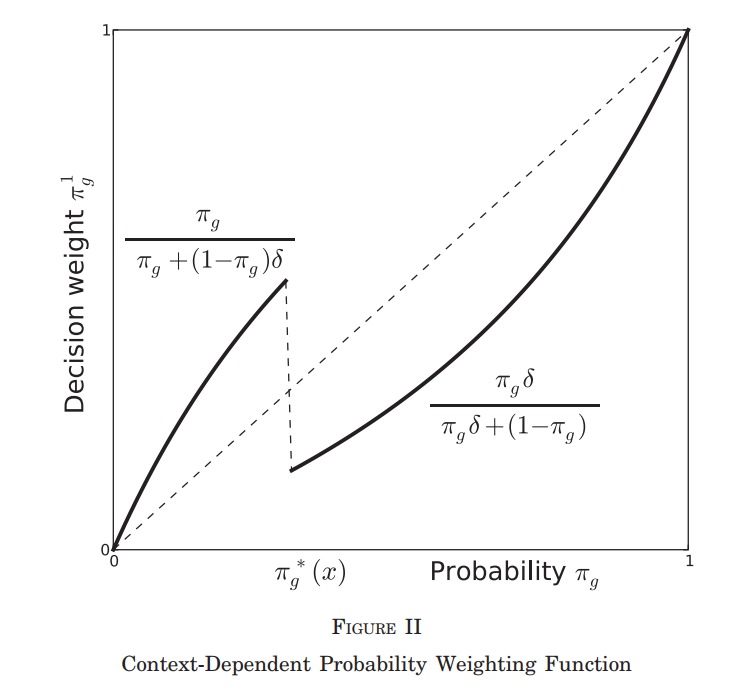
\includegraphics[width = 0.69\textwidth]{fig2.png}
\end{frame}


\begin{frame}{Risk attitudes:}
    \begin{definition}[3]
        A salience function is convex if, for any state with positive payoffs $(y, z)$ and any $x, \epsilon>0$,
        the difference $\sigma(y+x$, $z+x)-\sigma(y+x+\epsilon, z+x+\epsilon)$ is a decreasing function of the payoff level $x$.\\
        (concave if increasing in $x$).
    \end{definition}
    \begin{Lemma}[1]
        If the salience function is convex, then $r=v^{L T}\left(L_0\right)-$ $v^{L T}\left(L_1\right)$ weakly decreases with $x$.\\
        (concave if increases with $x$).
    \end{Lemma}
    $\Rightarrow$ if diminishing sensitivity weakens with $x$, a higher payoff level raises the relative attractiveness of  $L_1$.\\
    ($\pi_g^* $ increases, raises risk seeking)
\end{frame}

\begin{frame}{Some critical remarks:}
    \begin{itemize}
        \item Kontek (2016, EL): certainty equivatent not necessarily defined\medskip
        \item monotonicity for $N>2$ violated\medskip
        \item mixed experimental evidence if estimated from indifference curves\medskip
        \item also strong empirical support\medskip
        \item $\Rightarrow$ room for research\medskip
	\end{itemize}
\end{frame}


\end{document}
